\chapter{Annotation~Experiments}
\label{chap:annotation} 

In this chapter I demonstrate the practical use of the annotation tool by annotating 10 different datasets. 

\begin{figure*}[h!]
\centering
\begin{subfigure}[t]{1.0\linewidth}
  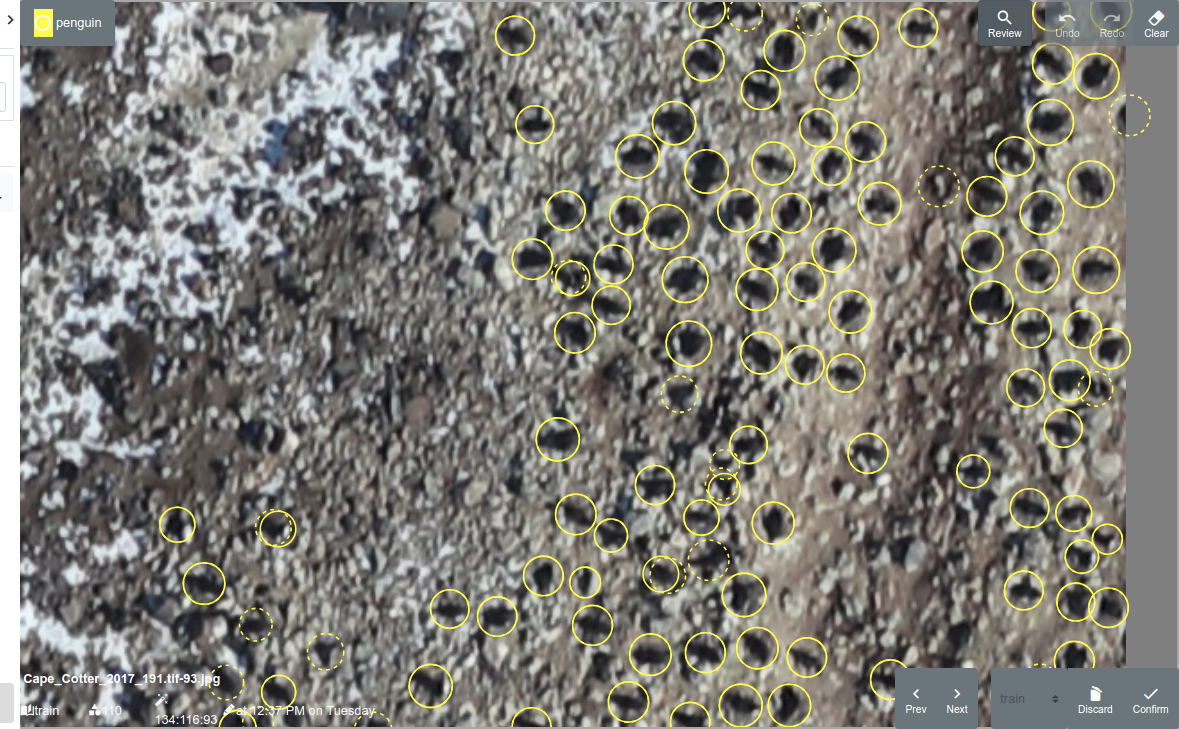
\includegraphics[width=0.475\linewidth]{figures/annotation/screenshots/penguins_aerial.png}
    \caption{}
 \end{subfigure}
 
\end{figure*}[h!]

\section{Datasets}

The datasets comprise a mix of relatively small scale image sets annotated for the sake of evaluating and developing the annotation method, image sets as test cases for future projects and a particular niche which seems suited to this kind of annotation method which is counting wildlife. In each case annotation time was between around an hour to around eight hours for the largest.





\section {Evaluation methods}
\label{sec:ann_evaluation}

The primary method of evaluation used in this work is that of \emph{continuous testing} whereby it is possible to see how the annotation process changes over time; how the model's predictions impact on the actions taken by the annotator, the type of actions and time required, and the accuracy of the model's predictions.

User edits are logged, along with predictions provided by the model (the starting point for annotating each image), and the final set of annotations submitted by the user. The accuracy of detections are verified directly by the user, giving both continuous testing of the model predictions as well as providing useful feedback to the user of the system. 

The types of actions as well as the timing can provide useful clues as to the difficulty of the task, and the level of assistance provided by the object detection model.


\subsection{Measuring progress}
\label{sec:ann_time}

\begin{figure*}[h!]
\centering
\begin{subfigure}[t]{1.0\linewidth}
  \includegraphics[width=0.475\linewidth]{charts/summaries/}
    \caption{}
 \end{subfigure}
 
\end{figure*}[h!]

Measuring progress over the period of annotating a dataset. Due to the variation between images, the granularity of recorded annotations (often several hundred per image) the raw actions need to be grouped in periods of time (for example, histograms). There are several ways progress could be measured, such as the time spent since annotation began, the training time invested training a model, the number of images or annotations submitted or the focus of this chapter, annotation time, the time the user spends actively using the tool.

The annotation logs recorded in this chapter were not taken in a controlled experimental setting, although an effort was taken to be consistent, by focusing as much as possible at the task at hand and avoiding distraction. It was therefore necessary to detect breaks, which at times occurred during annotating an image. Any action was capped at a maximum 1 minute for this purpose, and longer actions were considered to include break time. Ideally this would have been detected directly in the tool by detecting lack of input or loss of focus, and future studies will take this approach.



\section {Overview}

\subsection {Size distribution}

\begin{figure}[ht]
\centering
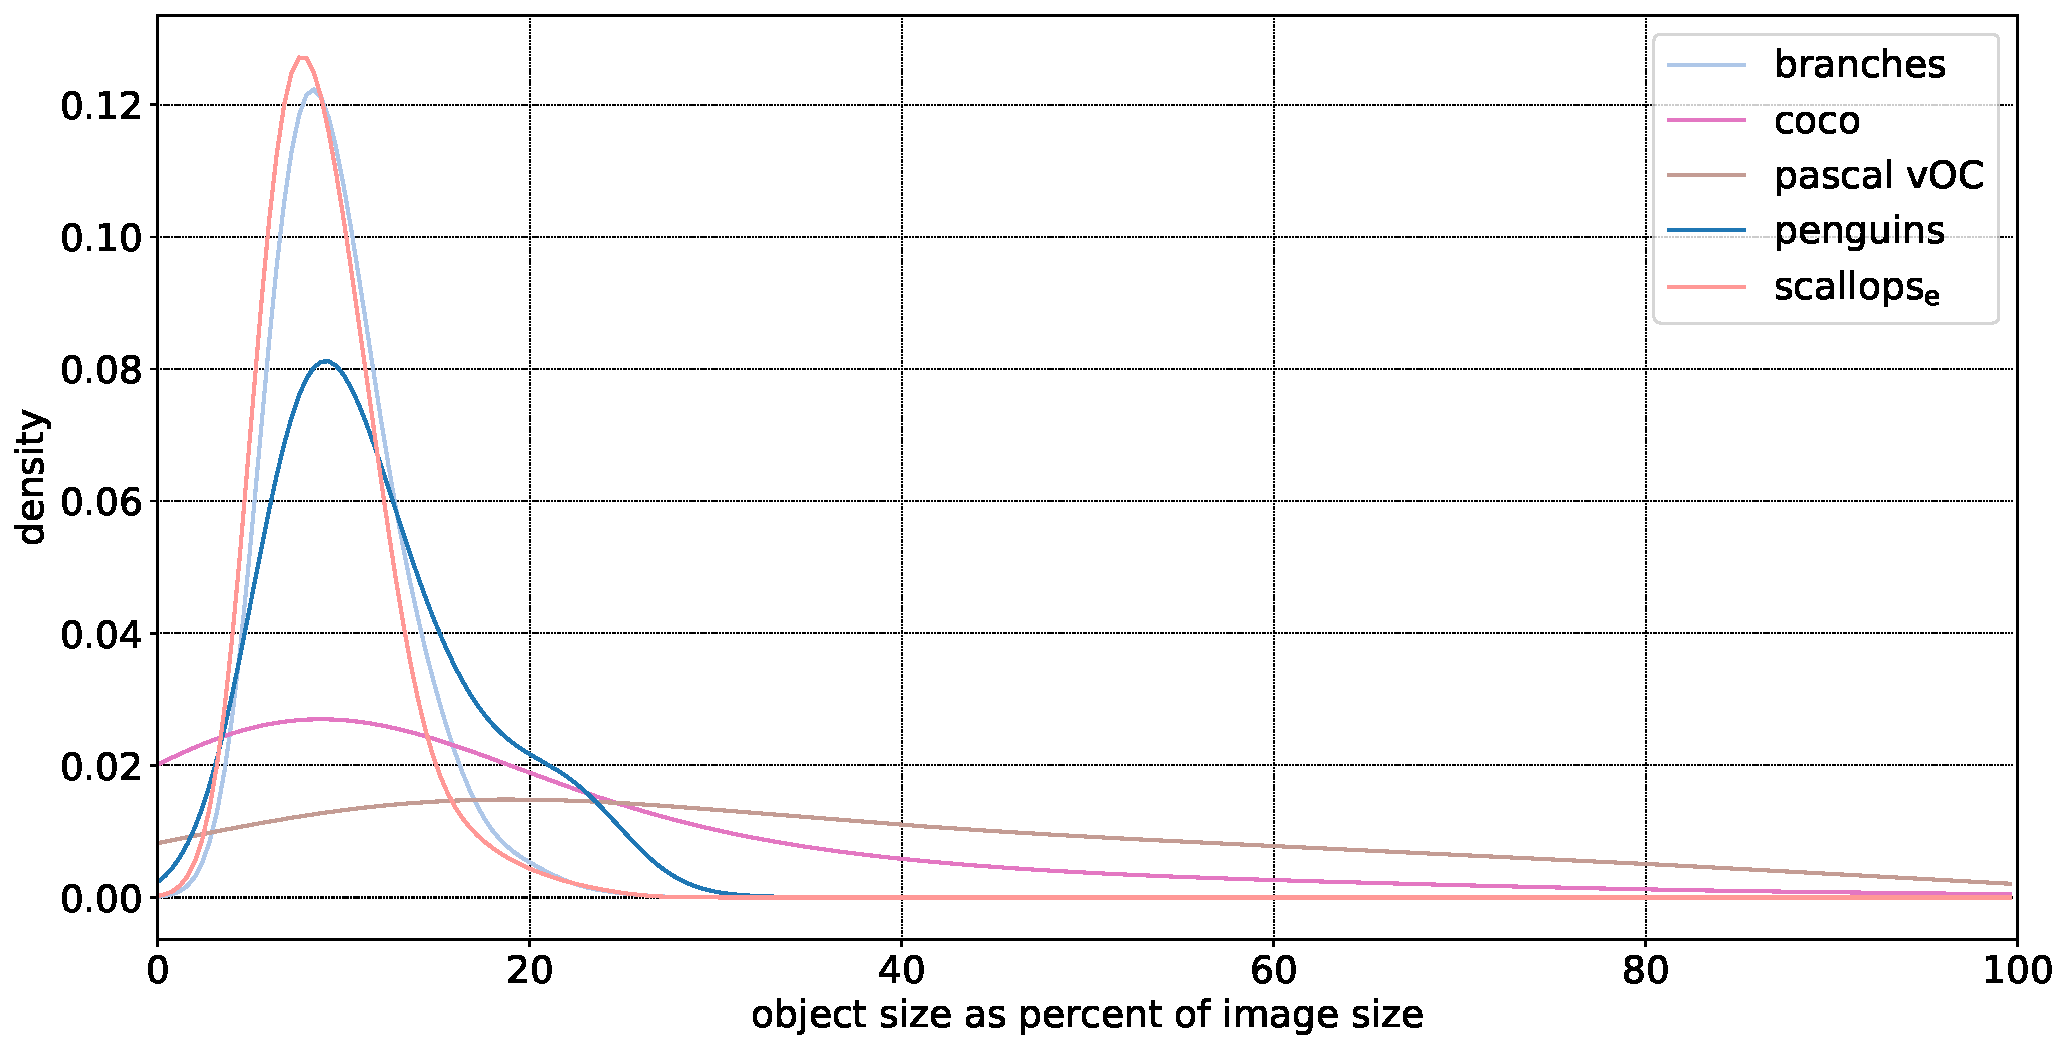
\includegraphics[width=1.0\linewidth]{charts/summaries/sizes_density.pdf}
\caption{Object bounding box size distributions as percent object to image size (average of width and height ratios) }
\label{fig:box_sizes}
\end{figure}


\begin{figure}[ht]
\centering
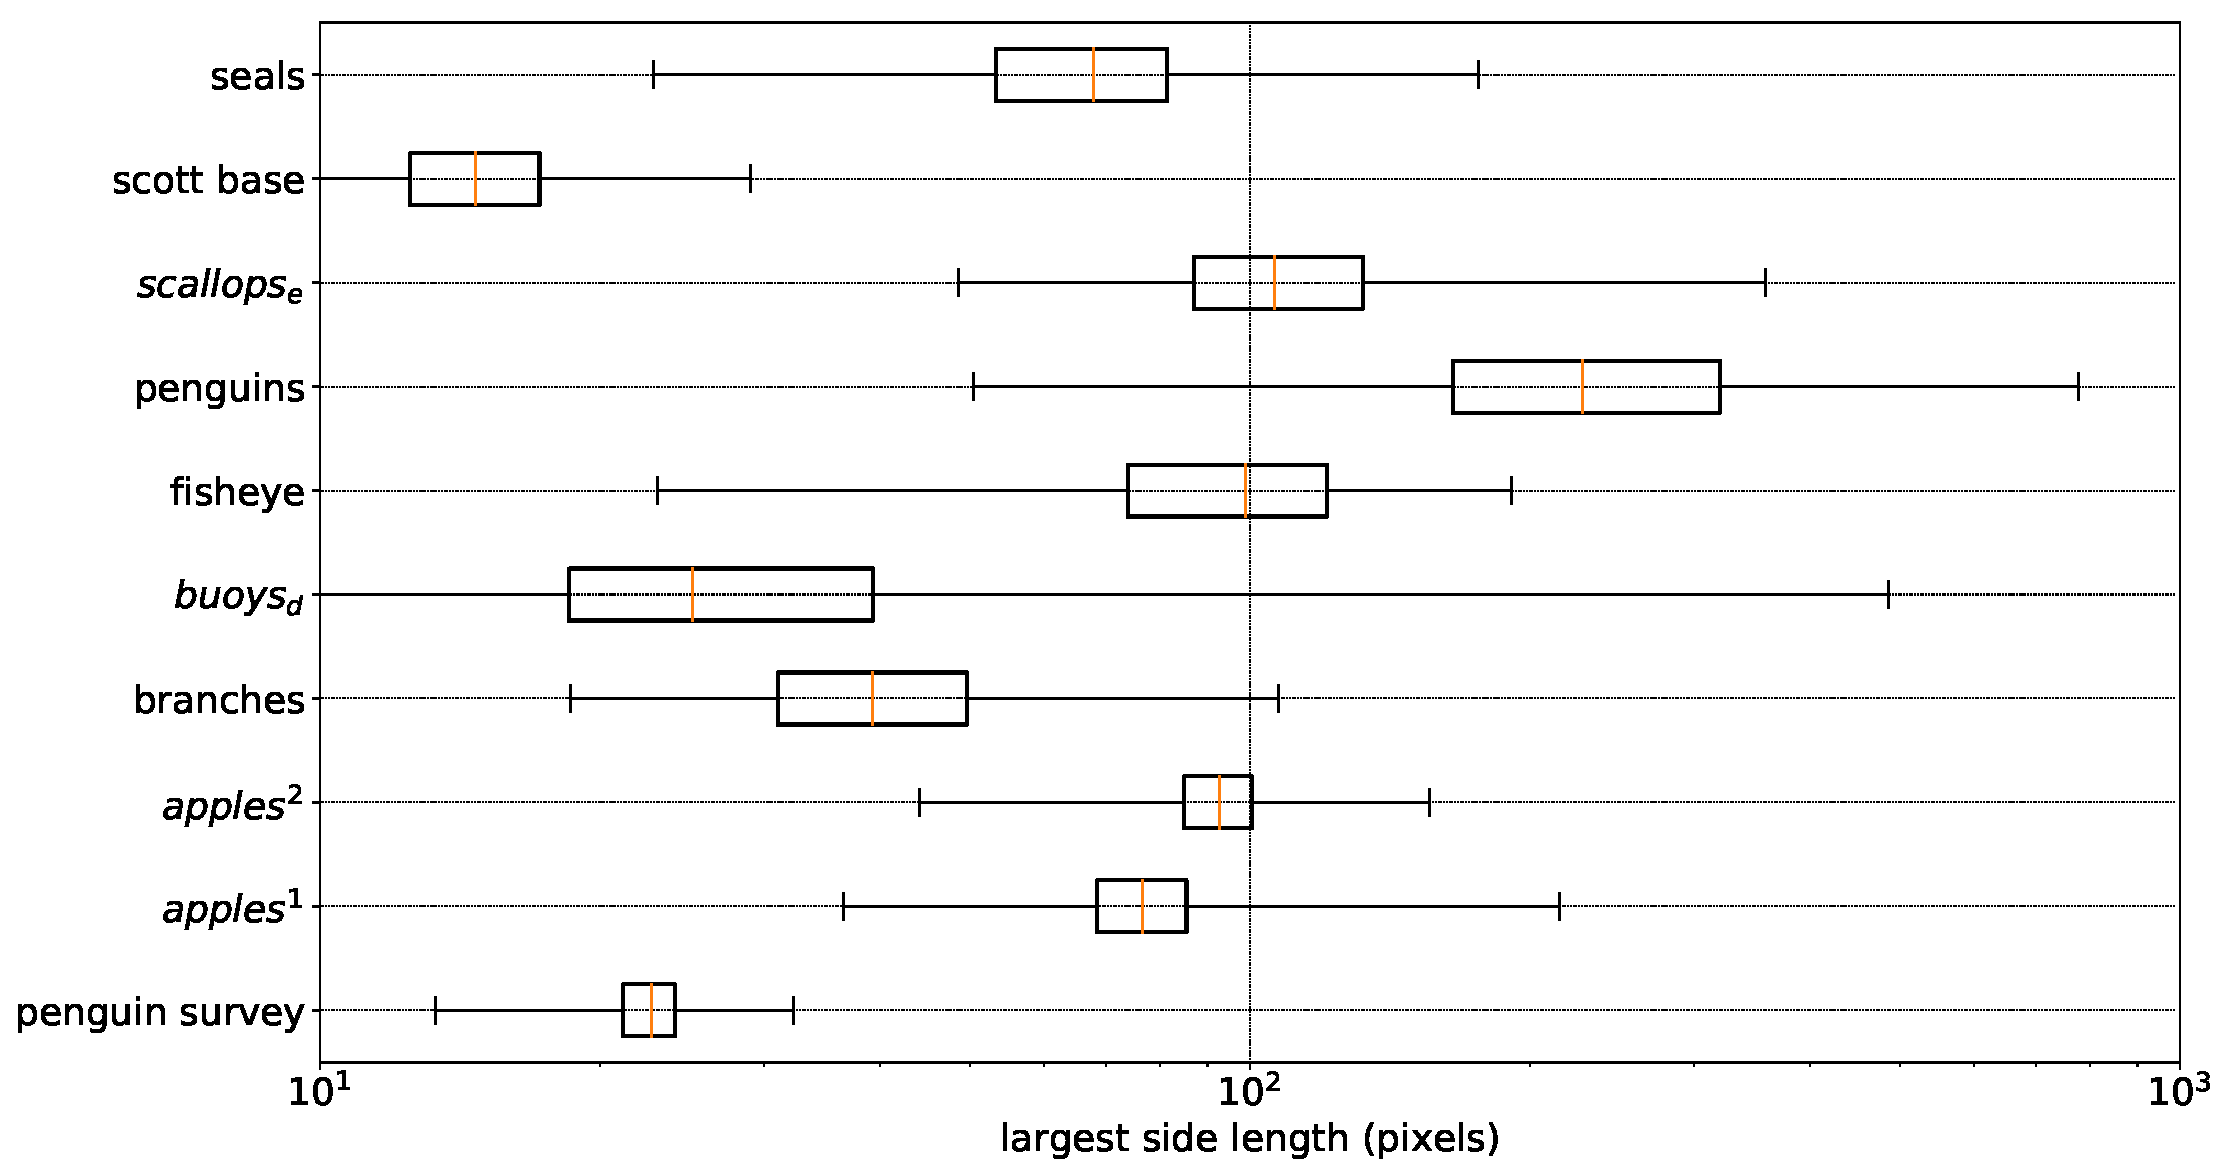
\includegraphics[width=1.0\linewidth]{charts/summaries/sizes_boxplot.pdf}
\caption{ Sizes in pixels of boxes for all annotated datasets }
\label{fig:box_sizes_plot}
\end{figure}

The sizes of objects in these datasets in general are small compared to more mainstream object detection datasets. This can be seen in figure~\ref{fig:box_sizes}, where compared to the Pascal VOC \cite{Everingham2008}, or COCO \cite{Lin2014}, the box sizes are smaller compared to the image size and less widely distributed. 

Figure \ref{fig:box_sizes_plot}  shows the object sizes (in pixels) of all the datasets together for comparison. In particular, the \emph{aerial penguin} and \emph{scott base} datasets have particularly tiny objects (not shown on the figure in order to preserve the scale). It can be seen that although the box sizes are relatively small in terms of the relative size to the image that at full resolution the objects can be relatively large in pixels.

Two different types of annotations are used in the annotations of these datasets. Circular annotations are used for very small objects and for counting objects where precise localisation is of less concern; circular annotations are also used for apples where it just happens to match the object shape well. The difference to the object detector is little, instead of estimating two parameters, width and height it is simply a radius. In all other respects a circle is treated as a square for computations such as \gls{IOU} overlap.

\subsection {Instance distribution}

\begin{figure}[ht]
\centering
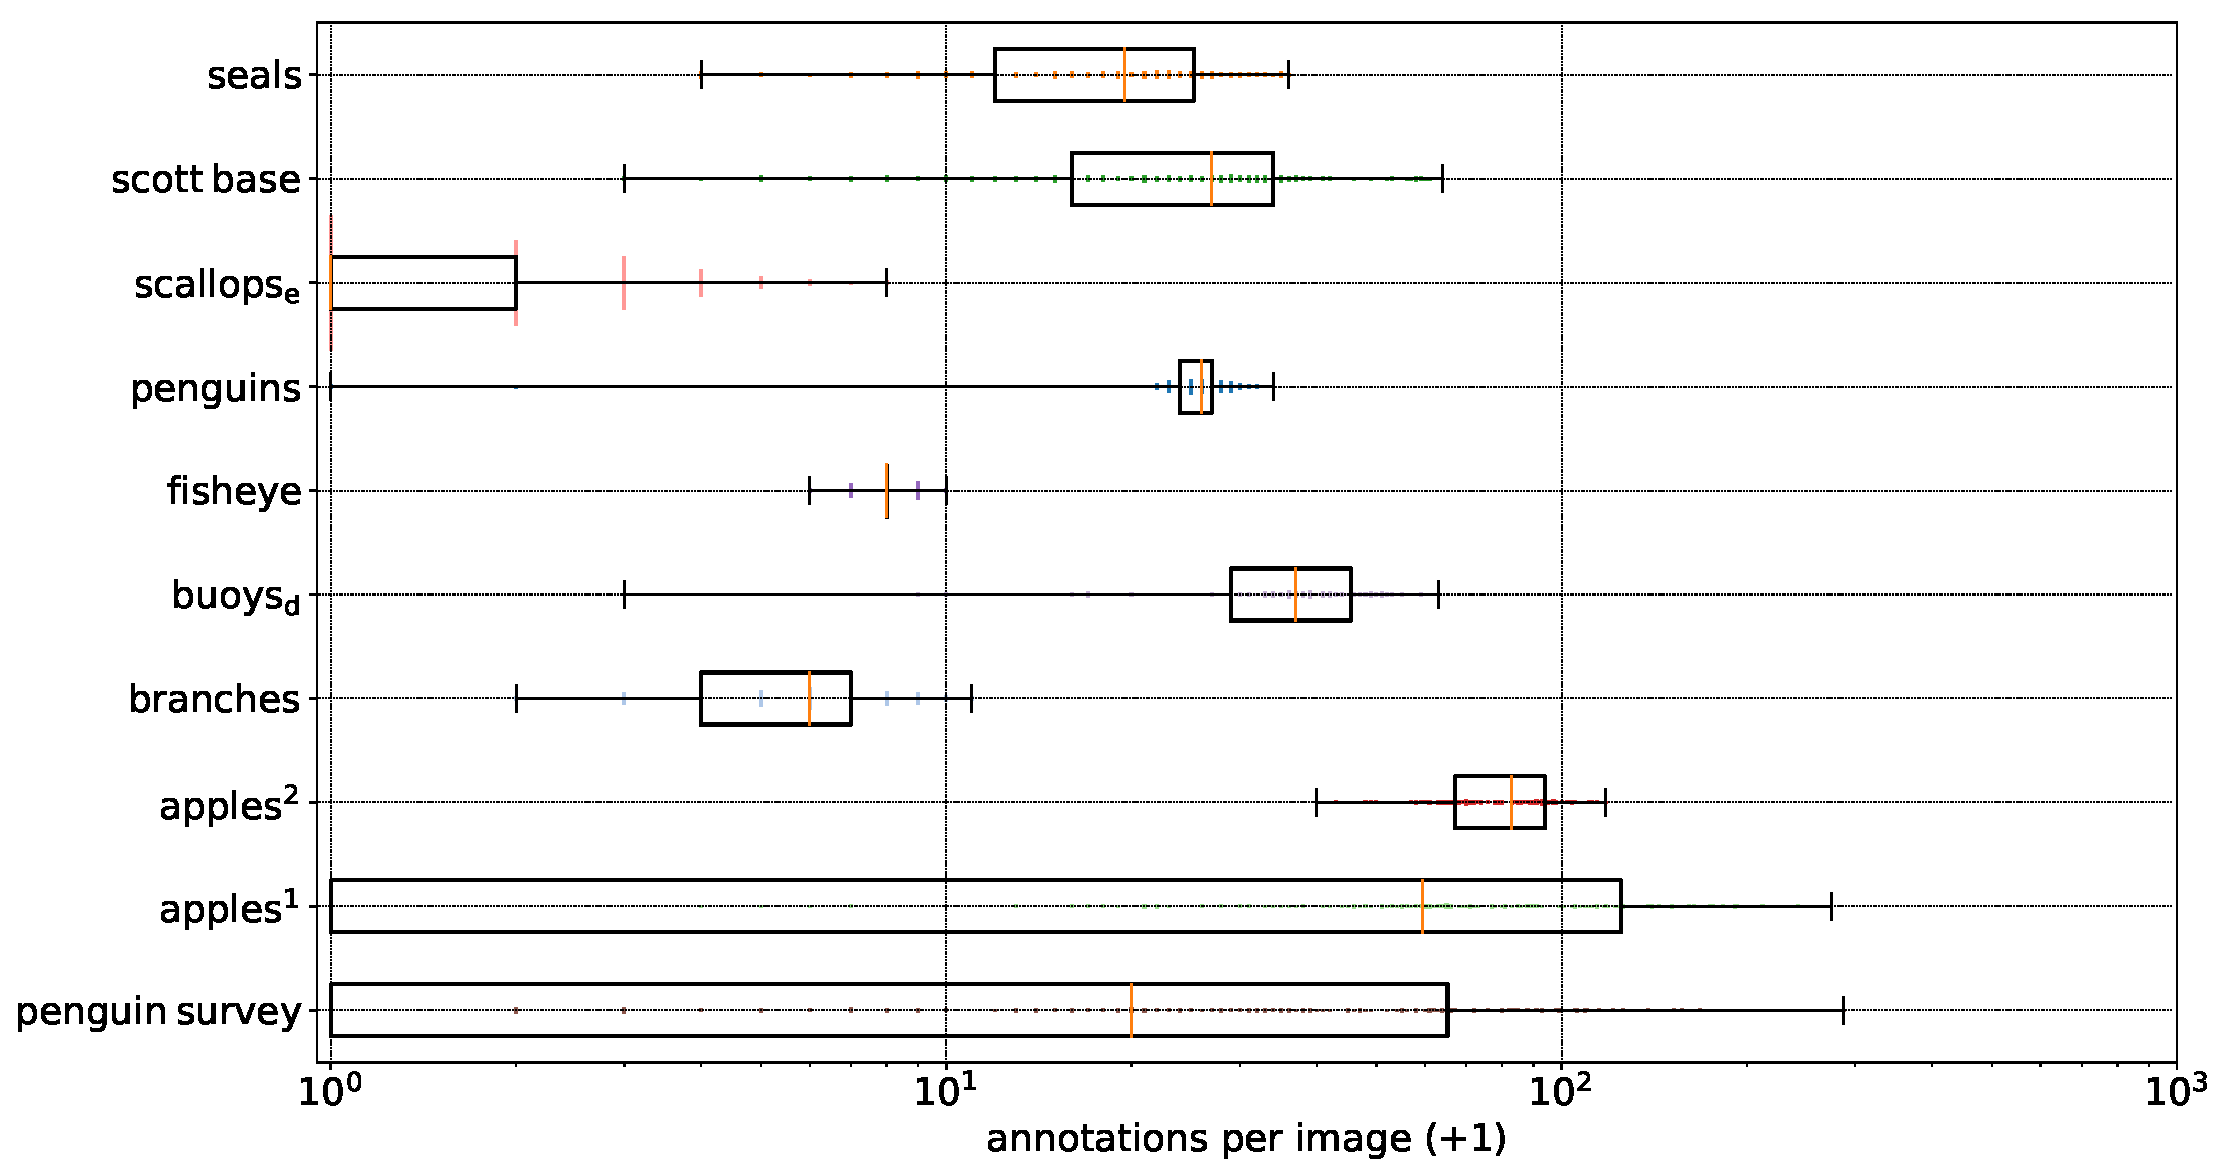
\includegraphics[width=1.0\linewidth]{charts/summaries/instances_boxplot.pdf}
\caption{ Distribution of object instances per image }
\label{fig:instances_image_plot}
\end{figure}

The datasets in question have a wide range of instance distributions, shown in figure~\ref{fig:instances_image_plot}. Some such as \emph{apples2}, \emph{branches} and \emph{fisheye} and \emph{penguins} contain a relatively uniform numbers of instances. Others especially \emph {aerial penguins}, \emph{scott base} and \emph{apples1} contain a wide range, a few with several hundred instances per image. One, \emph{scallops} contains very few instances and most images are negative images.


\section {Datasets}
\label{sec:datasets}

\section{Penguins}

\begin{figure*}[h!]
\centering
\begin{subfigure}[t]{1.0\linewidth}
  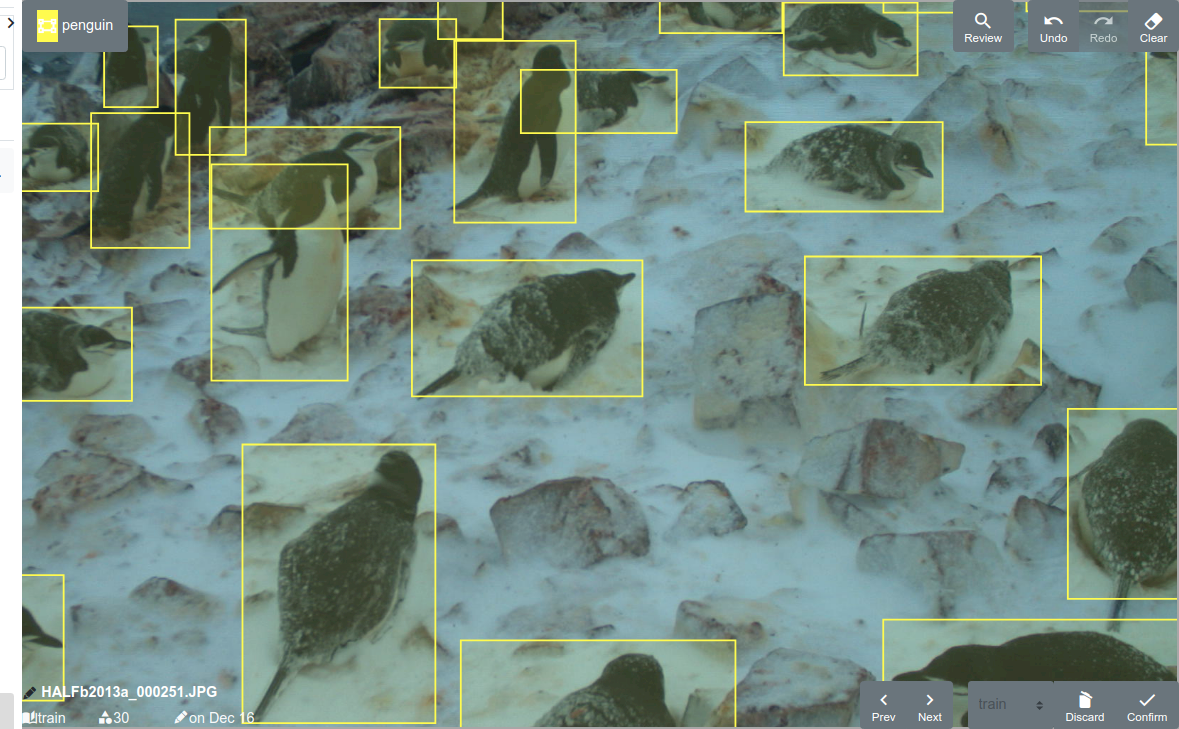
\includegraphics[width=0.475\linewidth]{figures/annotation/screenshots/penguins.png}
  \hfill
  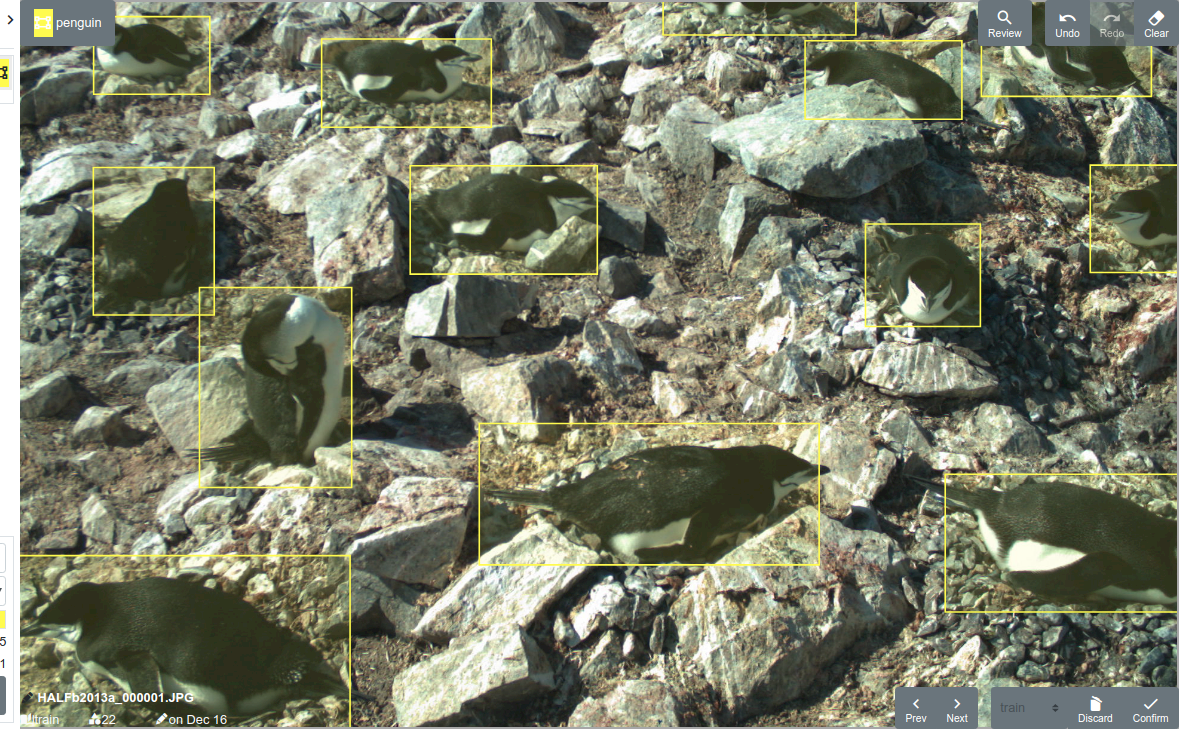
\includegraphics[width=0.475\linewidth]{figures/annotation/screenshots/penguins2.png}
\end{subfigure}

\caption{Example images from the \emph{penguin} dataset, \cite{PenguinData}, used primarily for testing and development}
\label{fig:penguin_dataset}
\end{figure*}

A dataset used in the development of the annotation tool, primarily because the object detector performed well on the images after only a few annotated images and the relative uniformity of the images. The images used are a subset of the \emph{penguin dataset} \cite{PenguinData} used for counting using point annotations \cite{Arteta2016}. Originally these annotations were created from multiple people using the Zooniverse crowd sourcing platform \cite{Zooniverse}. 

Specifically the images annotated in this work (examples seen in figure~\ref{fig:penguin_dataset} were from the 'HALFb' subset, taken from a fixed camera position over a period of time. Many images in this dataset contain complex overlapping instances, however in the 'HALFb' there is a small amount of overlapping but for the most part the standard anchor box object detector has no trouble in detecting all of the instances.


\section{Apples}


\begin{figure*}[h!]

\begin{subfigure}[t]{1.0\linewidth}
  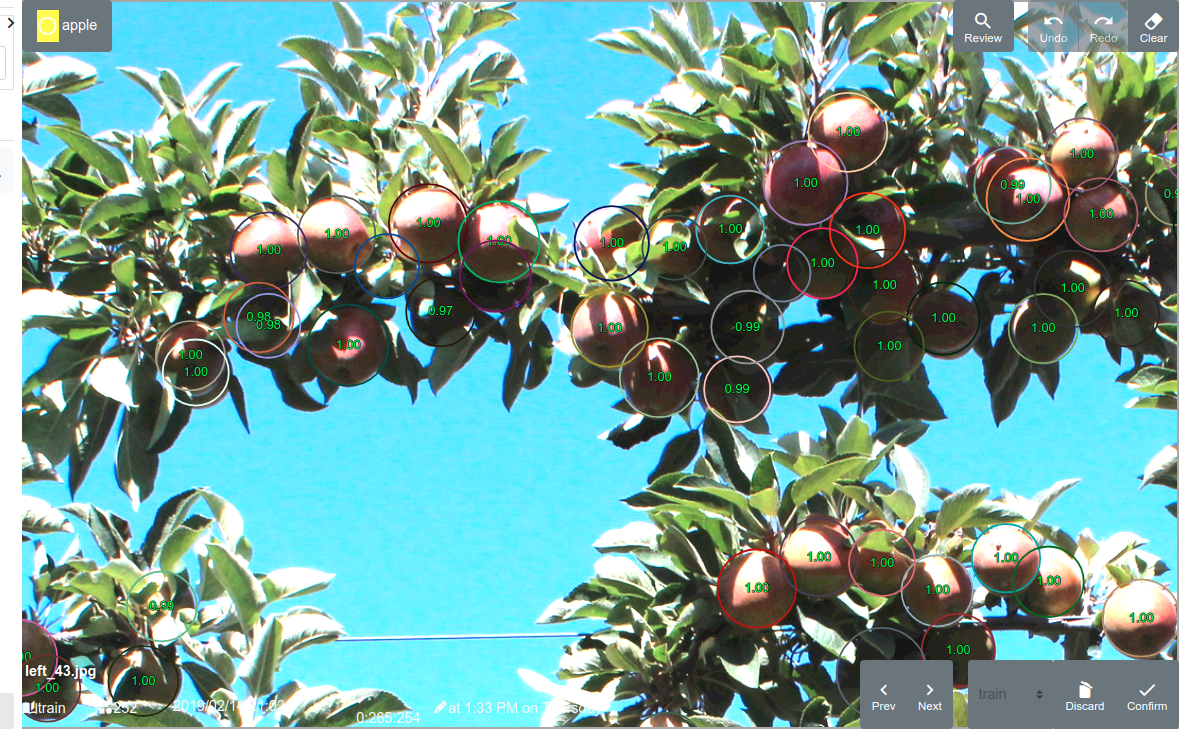
\includegraphics[width=0.475\linewidth]{figures/annotation/screenshots/apples_big.png}
  \hfill
  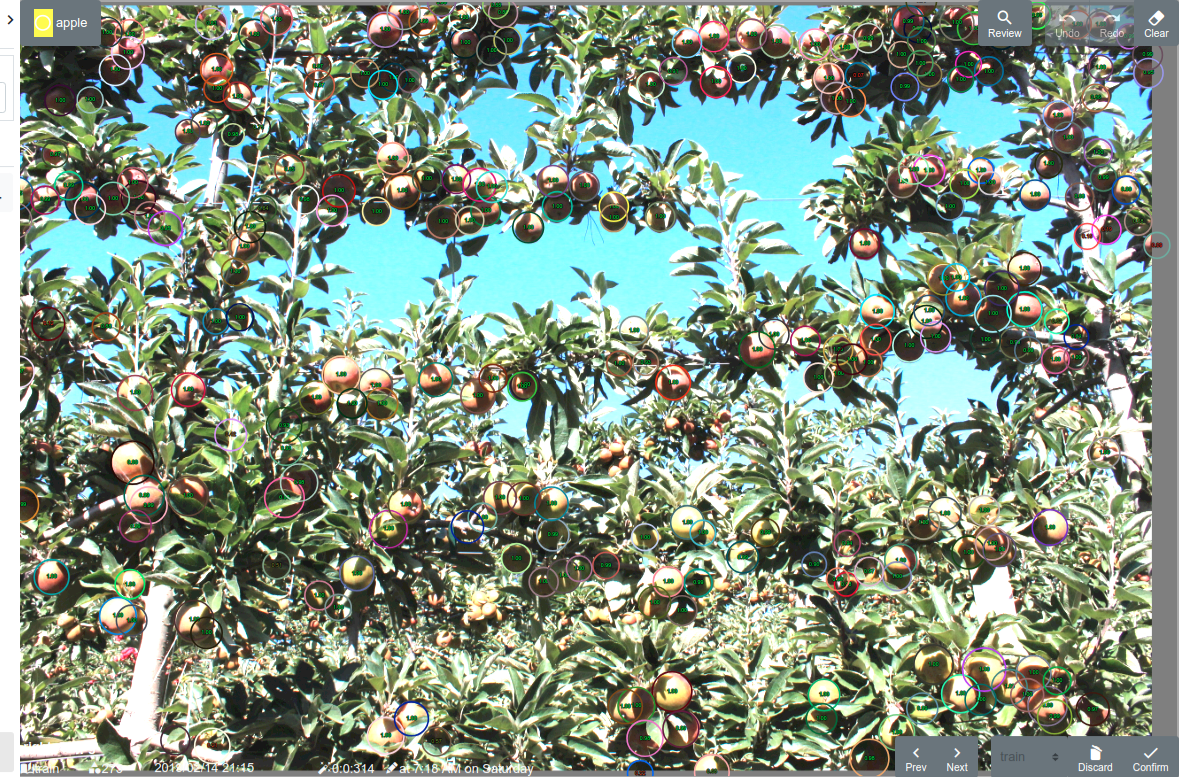
\includegraphics[width=0.475\linewidth]{figures/annotation/screenshots/apples_small.png}
\end{subfigure}
\caption{Example images from the \emph{apples1} and \emph{apples2} datasets}
\label{fig:apples_dataset}  
\end{figure*}


\section{Buoy}

\begin{figure}[h]
  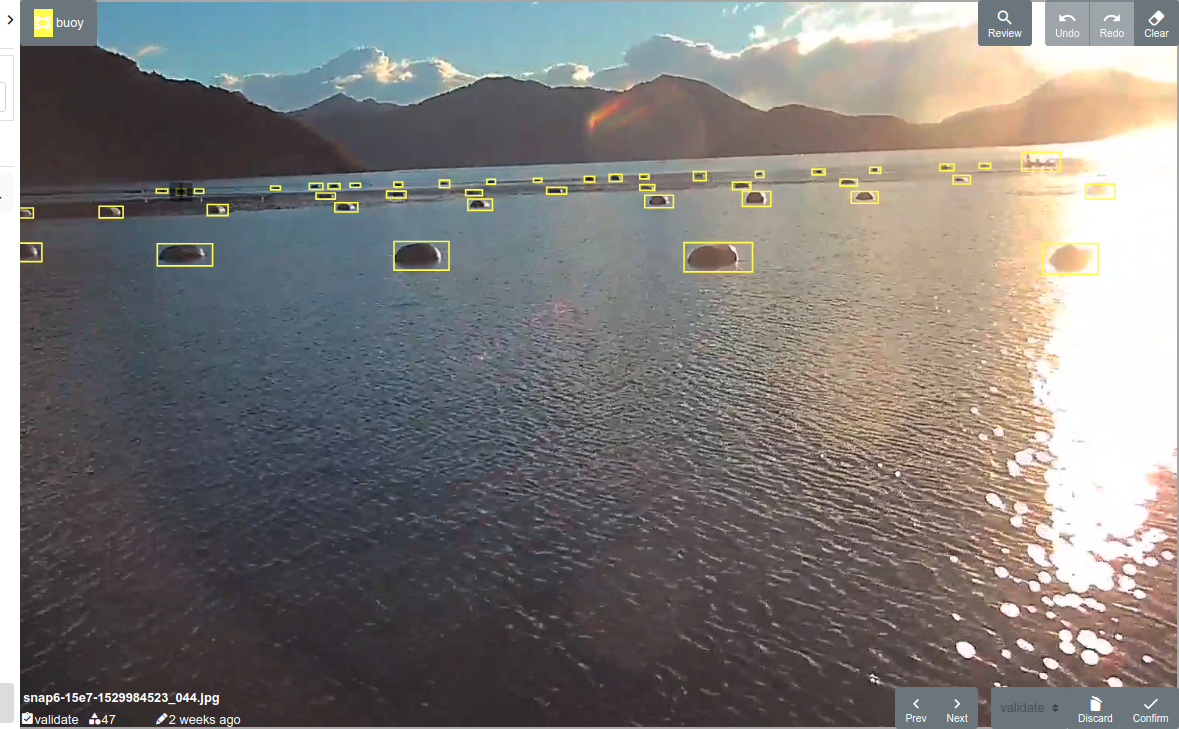
\includegraphics[width=0.5\textwidth]{figures/annotation/screenshots/buoys.png}
  \caption{Example image from the \emph{buoys} dataset of mussel farm buoys captured from a camera attached to another buoy }
  \label{fig:buoys_dataset}
\end{figure}

\section{Fisheye}

\begin{figure}[h]
  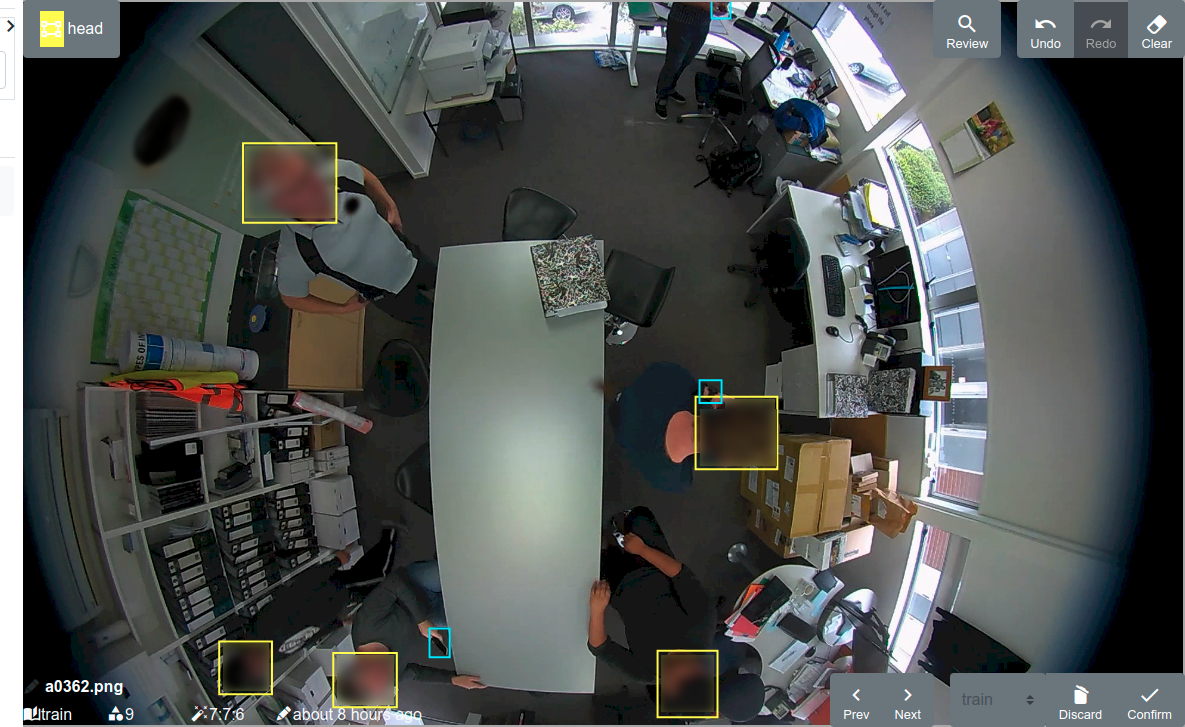
\includegraphics[width=0.5\textwidth]{figures/annotation/screenshots/victor.png}
  \caption{Example image from the \emph{fisheye} dataset of fish-eye lens head and cellphone detection }
\end{figure}

\section{Branches}


\begin{figure}[h]
  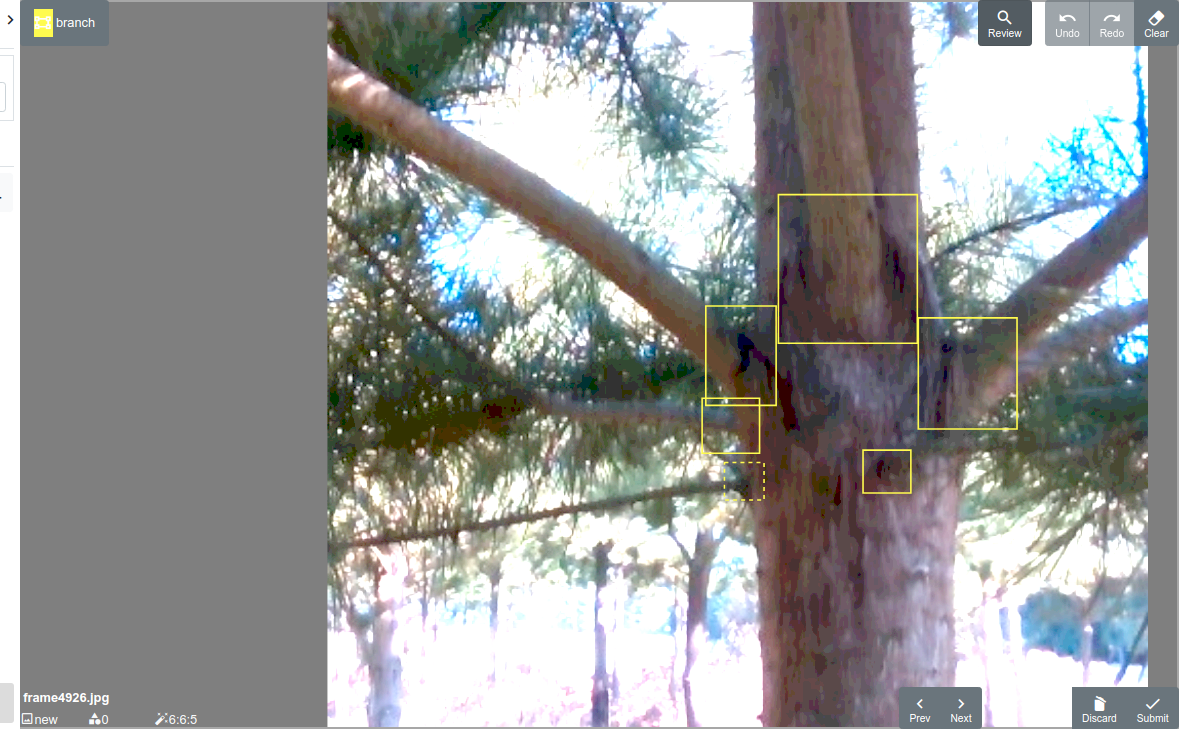
\includegraphics[width=0.5\textwidth]{figures/annotation/screenshots/branches3.png}
  \caption{Example image from \emph{branches}, tree branch intersection detection}
  
\end{figure}


\section {Scallop}

\begin{figure*}[h!]
\begin{subfigure}[t]{1.0\linewidth}
  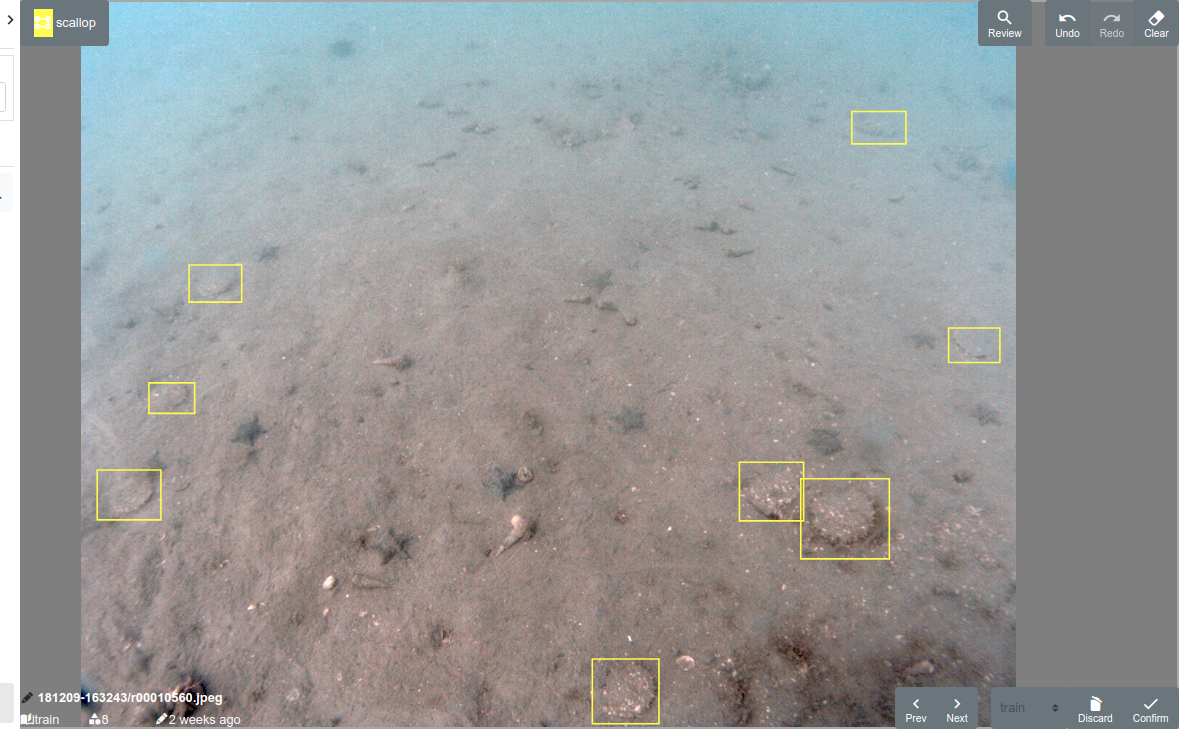
\includegraphics[width=0.475\linewidth]{figures/annotation/screenshots/scallops.png}
  \hfill
  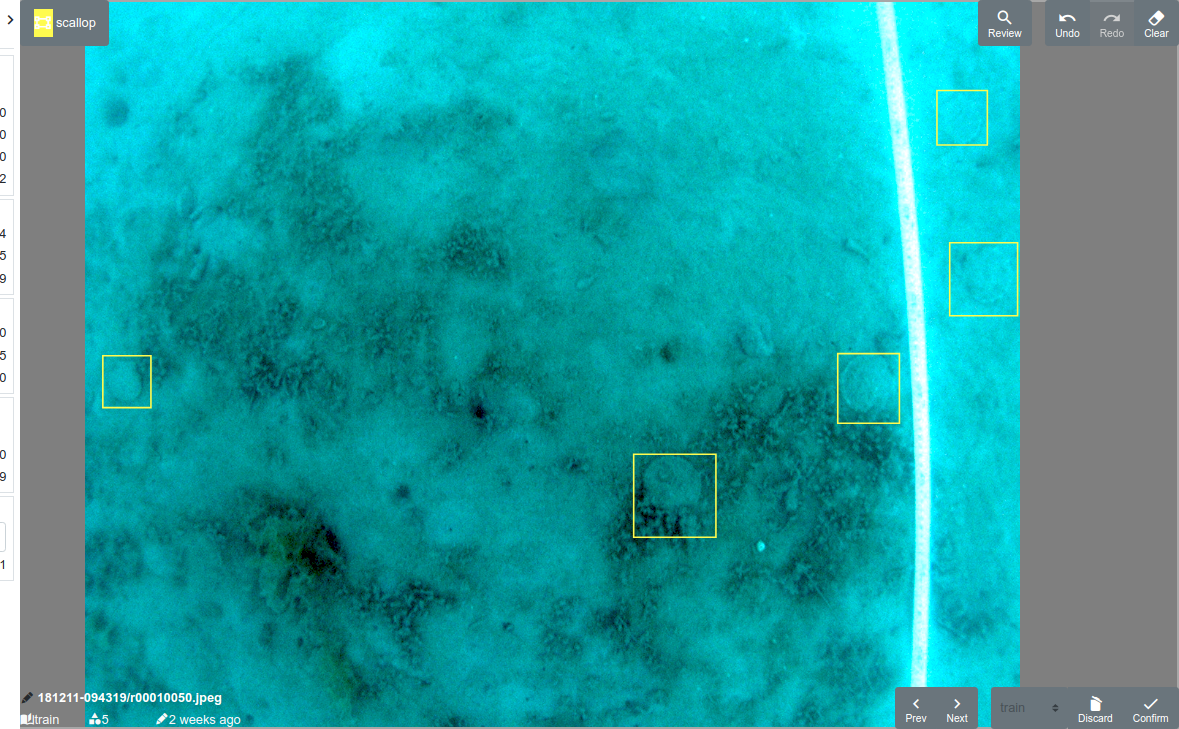
\includegraphics[width=0.475\linewidth]{figures/annotation/screenshots/scallops3.png}
\end{subfigure}

\caption{Example images from the \emph{scallop} dataset}
\label{fig:scallop_dataset}  

\end{figure*}



\section{Case study: counting Adélie penguins from aerial photographs}

\begin{figure*}[h!]
\centering
\begin{subfigure}[t]{1.0\linewidth}
  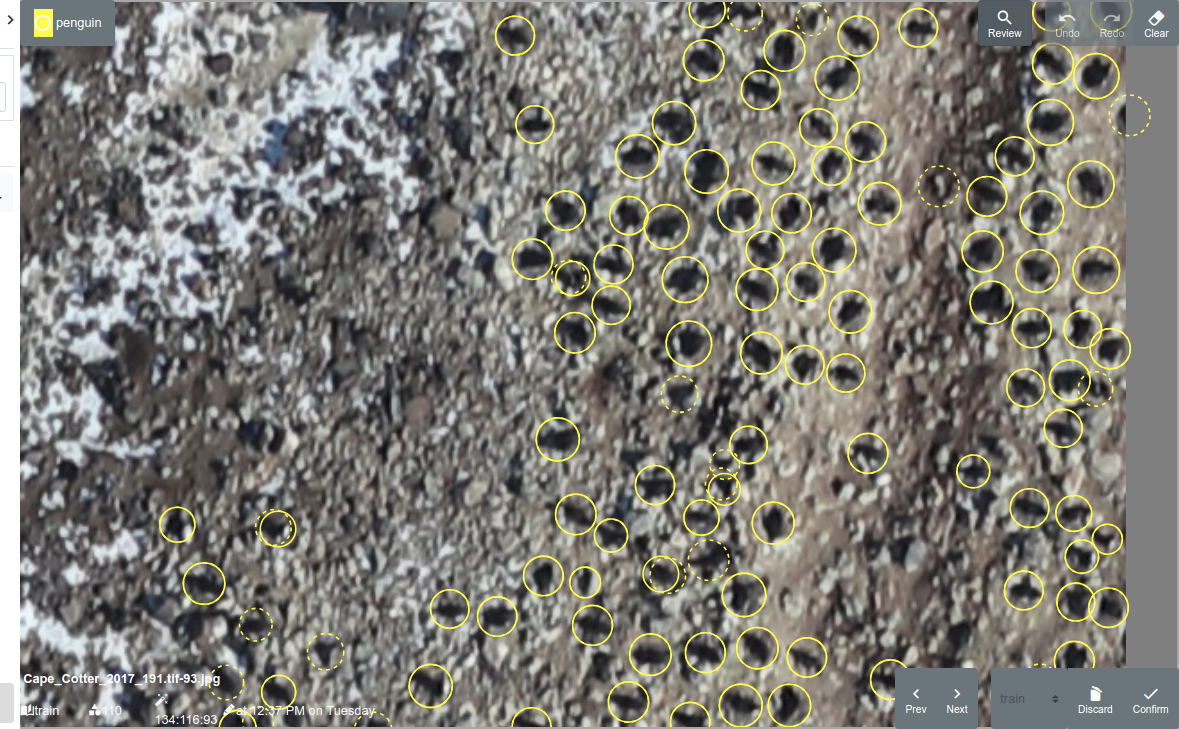
\includegraphics[width=0.475\linewidth]{figures/annotation/screenshots/penguins_aerial.png}
  \hfill
  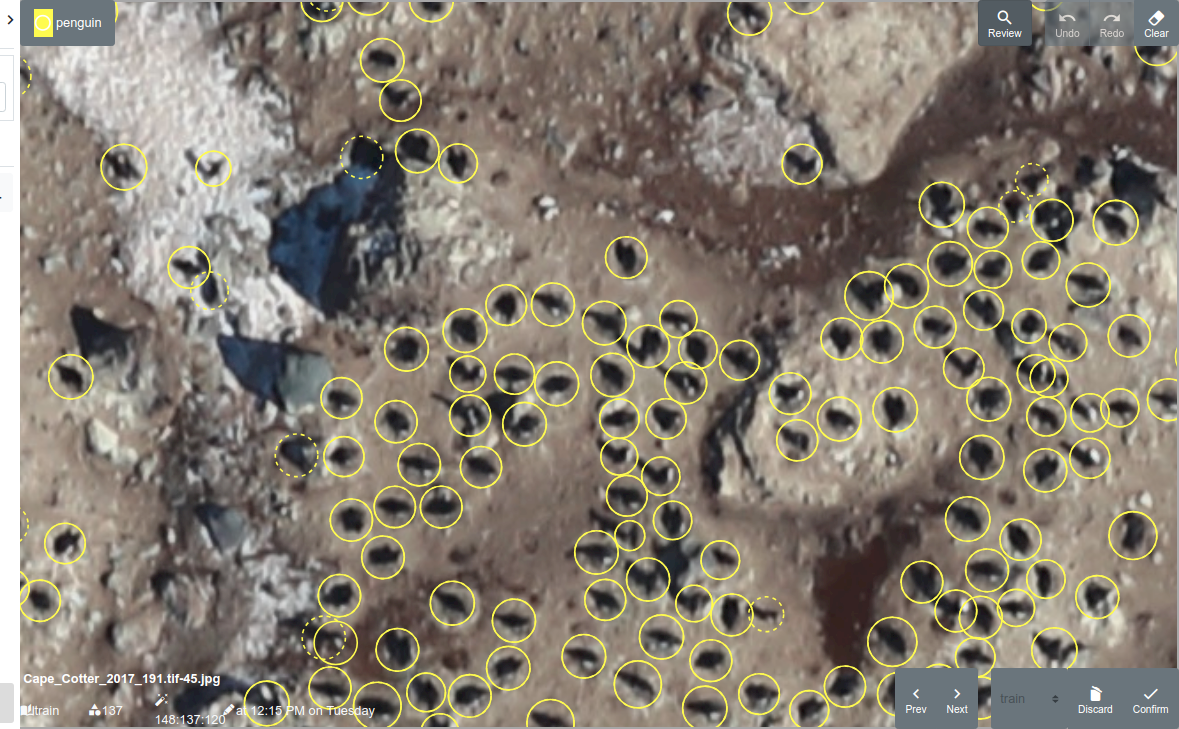
\includegraphics[width=0.475\linewidth]{figures/annotation/screenshots/penguins_aerial2.png}
  \caption{}
\end{subfigure}

\caption{ }
\label {fig:penguin_aerial_examples}
\end{figure*}

One potentially useful for verification based annotation is counting things, it provides some of the time savings of automatic inference but also the accuracy of human annotation because the machine predictions are verified, and can begin without possessing an existing dataset or developing specific recognition methods.


One of the sources of inspiration for this work in verification based annotation came from \cite{McNeill2011}, where a tool was created to semi-automatically count Adelie penguins from aerial photographs. The penguins are first automatically detected, then follows a verification process allowing a human annotator to mark false positives and false negatives.

The method for detecting penguins is to first detect penguin colonies which can be done many times by the unique colour of the penguin guano. Individual penguins were then identified by thresholding and local minima detection and culling of long thin objects. 

The images (two of which can be seen in figure~\ref{fig:penguin_examples}), originate from aerial photographic surveys \cite{Lyver2014}, from high resolution photographs, taken from 2000-2500 feet. In the case of the two images from Cape Cotter and Hallet in figure~\ref{fig:penguin_examples}, the images are cropped from images of size $ 6720\times4480 $. The Cape Royds images are spliced together from three images with various areas masked out, this was done by filling in the overlapping and irrelevant areas using a paint program.

The study which has been conducted from 1981 until present, prior to 2010 involved manually counting individual penguins using a pin to manually mark penguins and avoid duplication. 





\begin{figure*}[h!]
\centering
\begin{subfigure}[t]{1.0\linewidth}
  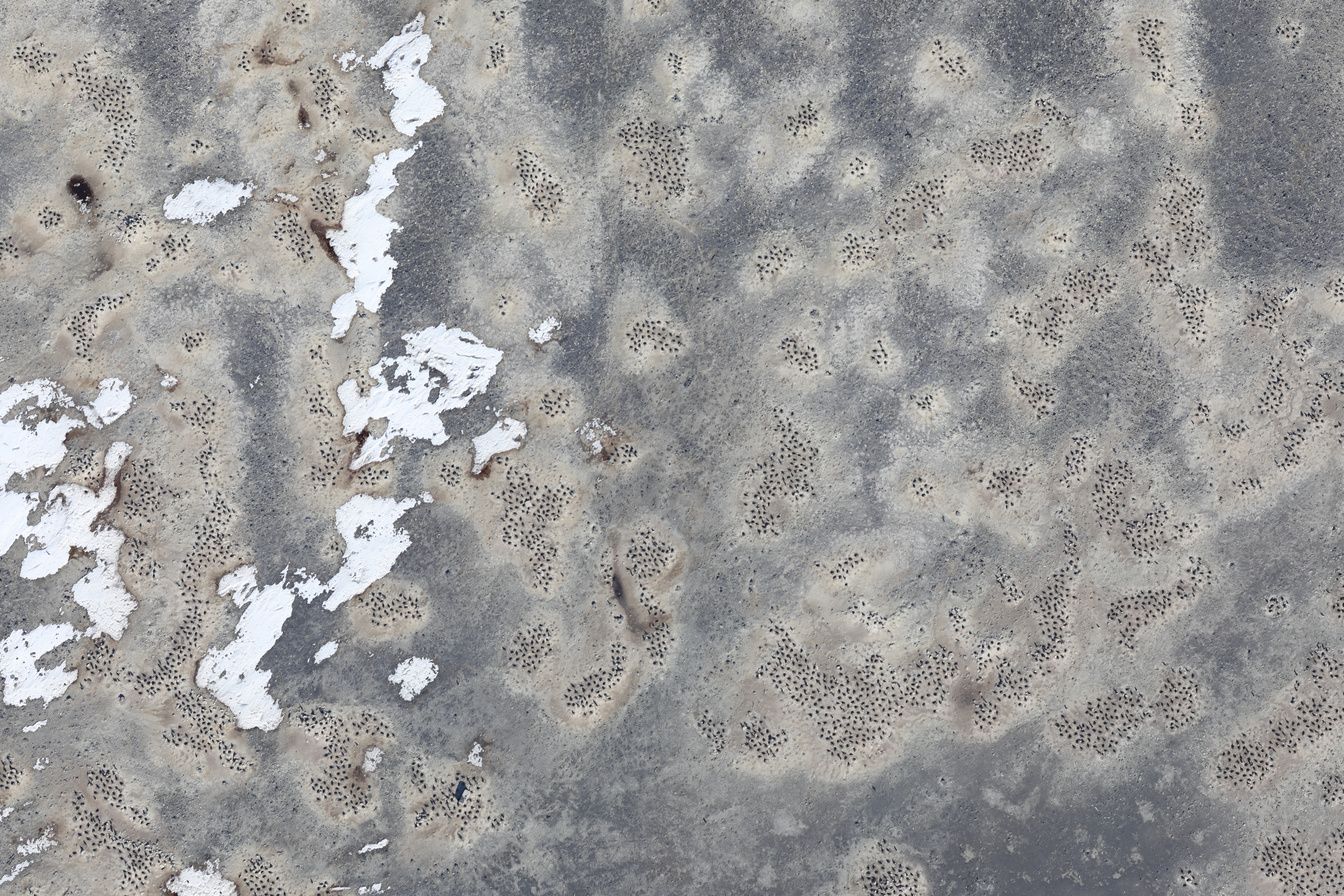
\includegraphics[width=0.475\linewidth]{figures/annotation/penguin/hallet_large.jpg}
  \hfill
  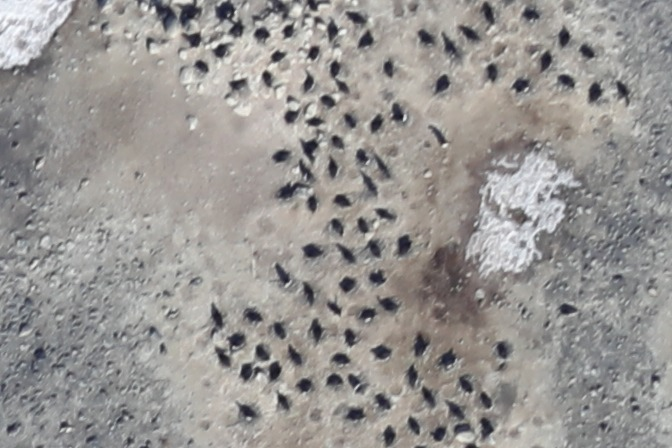
\includegraphics[width=0.475\linewidth]{figures/annotation/penguin/hallet.jpg}
  \caption{Cape Hallett 2017}
\end{subfigure}
\begin{subfigure}[t]{1.0\linewidth}
  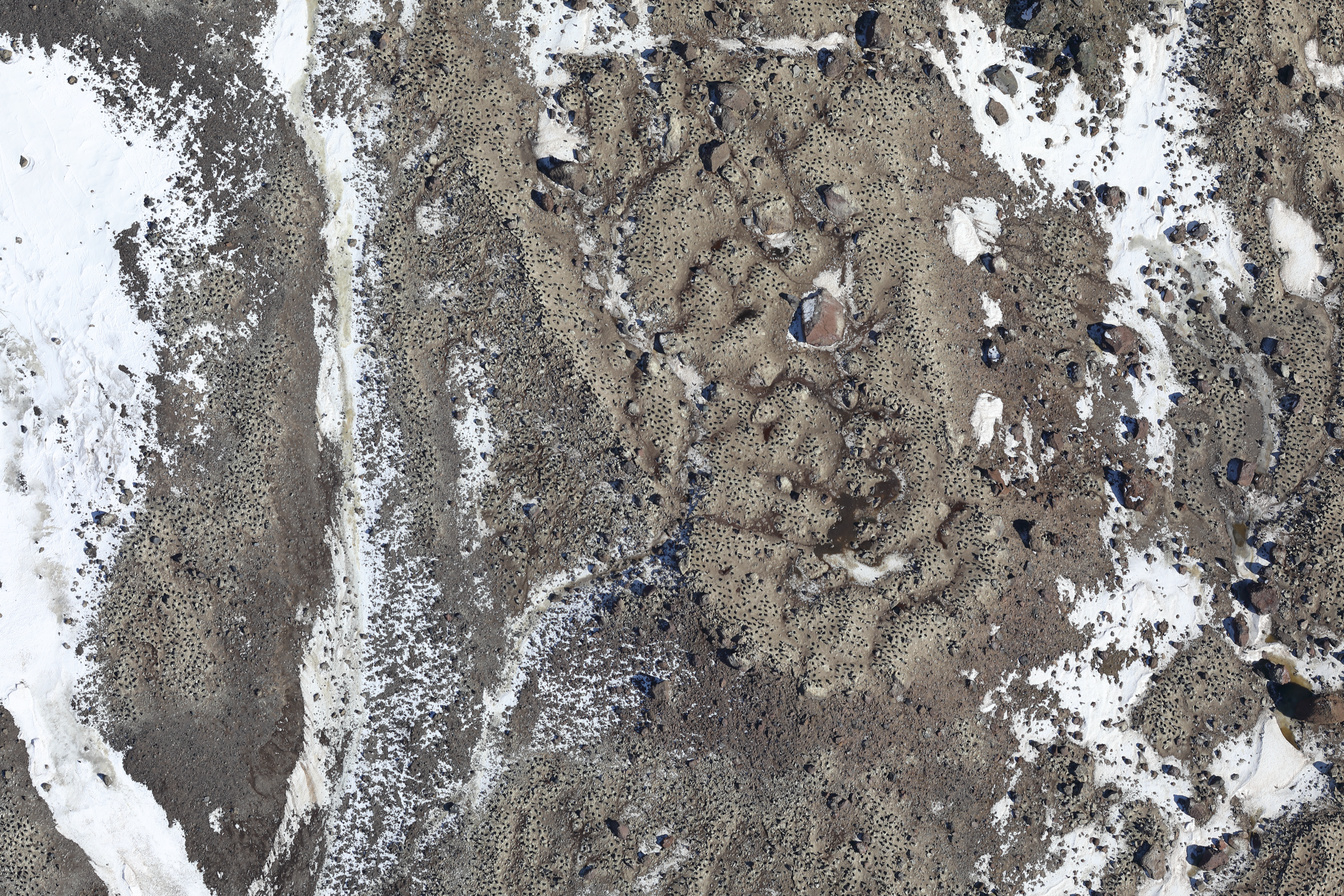
\includegraphics[width=0.475\linewidth]{figures/annotation/penguin/cotter_large.jpg}
  \hfill 
  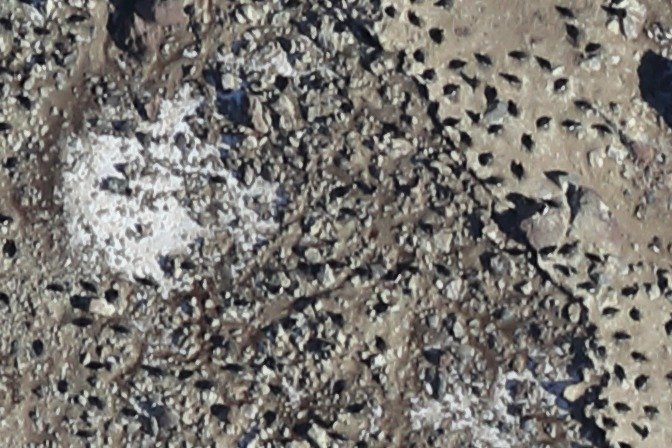
\includegraphics[width=0.475\linewidth]{figures/annotation/penguin/cotter.jpg}
  \caption{Cape Cotter 2017}
\end{subfigure}
\begin{subfigure}[t]{1.0\linewidth}
  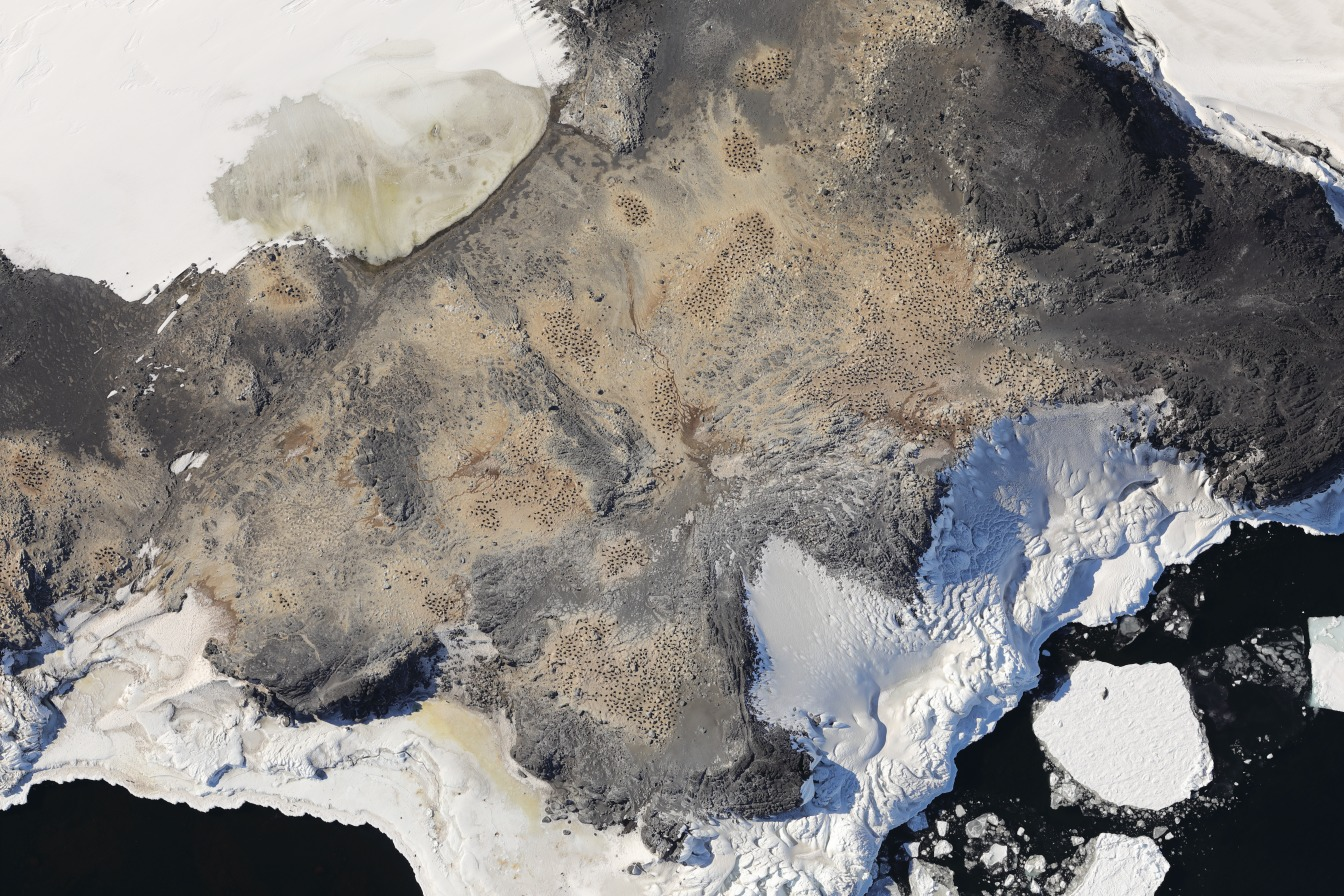
\includegraphics[width=0.475\linewidth]{figures/annotation/penguin/royds_large.jpg}
  \hfill
  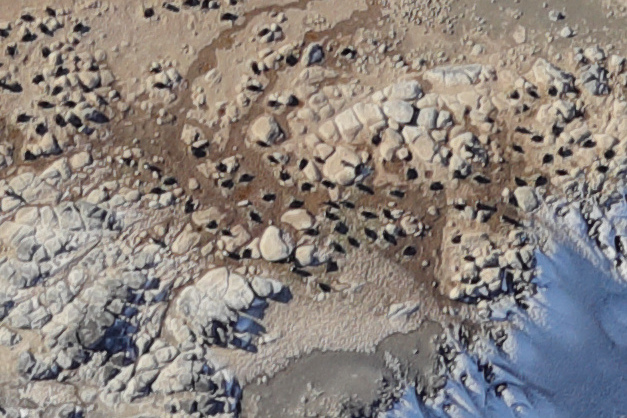
\includegraphics[width=0.475\linewidth]{figures/annotation/penguin/royds.jpg}
  \caption{Cape Royds 2017}
\end{subfigure}

\caption{Examples from the Adelie penguin census data taken in 2017. On the left hand column are images showing the zoomed out landscape, on the right are representative crops zoomed in.  In (a) an image from Cape Hallet image showing clearly visible, easy to identify penguins as dark patches. In (b) Cape Cotter showing many more difficult to identify penguins, often with a high degree of ambiguity not only for the machine learning algorithm but for a human annotator, in rocky areas especially shadows from rocks are very difficult to discern from penguins. In (c) Cape Royds, a smaller colony to the other two (and complete). In terms of ambiguity and uncertainty somewhere in-between. }
\label {fig:penguin_examples}
\end{figure*}


\subsection {Effect of uncertainty}

 The strength of the object detector has an effect on the usefulness of verification. If a detector is weak and the noise of many inaccurate detections overwhelms the number of any accurate detections, verification becomes less effective - and manual annotation becomes more efficient. When the source images are very uncertain this presents a challenge not only for the object detector which may be relatively weaker as a result, but for the human annotator. Many of the penguin instances to the untrained eye appear very similar to the shadow cast by rocks and difficult to discern. The nature of the imagery from the different sites shown in figure~\ref{fig:penguin_examples} provide a test case to compare the effectiveness of verification with different levels of uncertainty in the source image. 

\subsection {Method}

Separately I annotated the three sets of penguins using the annotation tool. I used circular annotations as the precise location of the penguins is of no consequence for counting applications, and in general the penguins separate themselves with a wide berth (when viewed from above).  

The very large original images were split into images of size $ 672\times448 $ (Cape Royds images were of similar size, but not exactly the same because the source images were of different size, rather than one big image like the other two). Image crops of those image, sized $ 300\times300 $ were then used during training.

\begin{table}[ht]
  \centering
    \caption{Statistics from the thee penguin sources. }
  \begin{tabular}{ l  l  l  l  l }
    Image set & Total & Images & Validation & $AP_0.5$ \\
    \toprule
    Cape Hallett  & 4217 & 100 & 683 & 0.97 \\
    Cape Cotter   & 6180 & 100 & 973 & 0.72  \\
    Cape Royds    & 2754 & 61 & 477  & 0.88 \\
    \bottomrule
  \end{tabular}

\label{fig:penguin_statistics}
\end{table}





\subsection{Results and discussion}
 
The difference in difficulty can clearly be seen in the difference of mAP in figure~\ref{fig:penguin_statistics}, where the Cape Hallet penguins were detected with almost perfect accuracy, whereas Cape Royds was more difficult and Cape Cotter considerably more difficult. 





\subsection{Case Study: Analysing Waddell Seal Counts}



\begin{figure*}[h!]
\centering
\begin{subfigure}[t]{1.0\linewidth}
  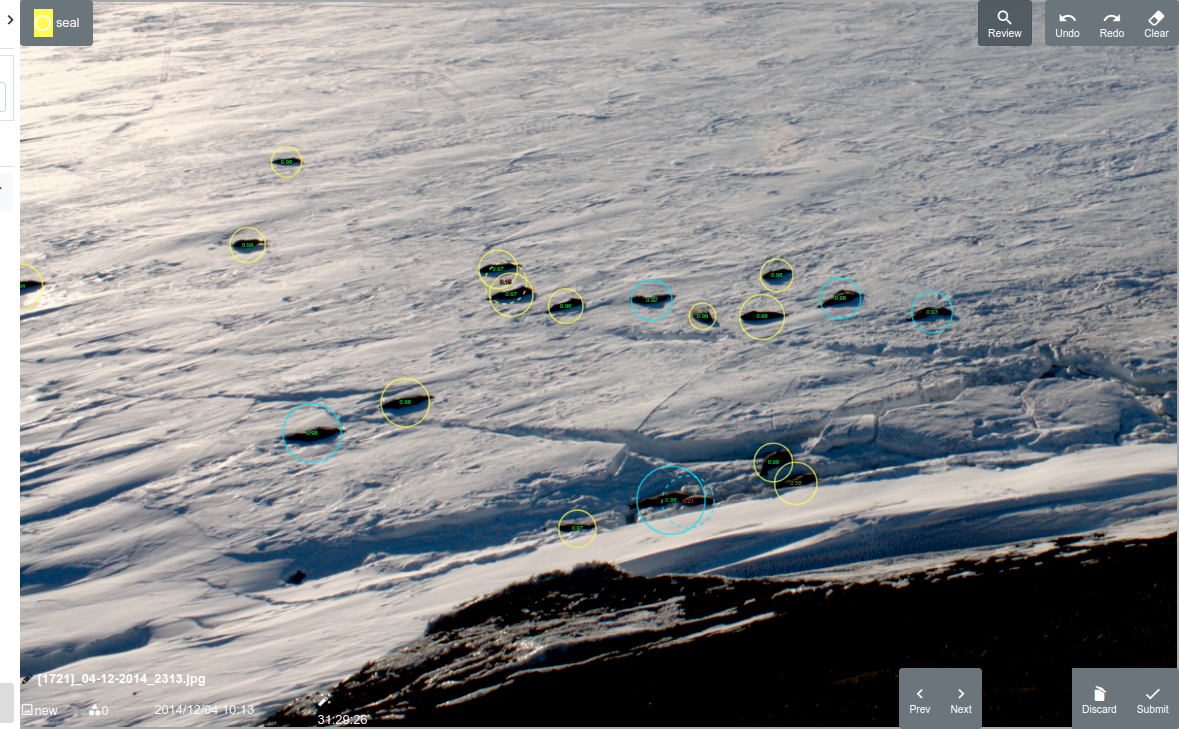
\includegraphics[width=0.475\linewidth]{figures/annotation/screenshots/seals_small2.png}
  \hfill
  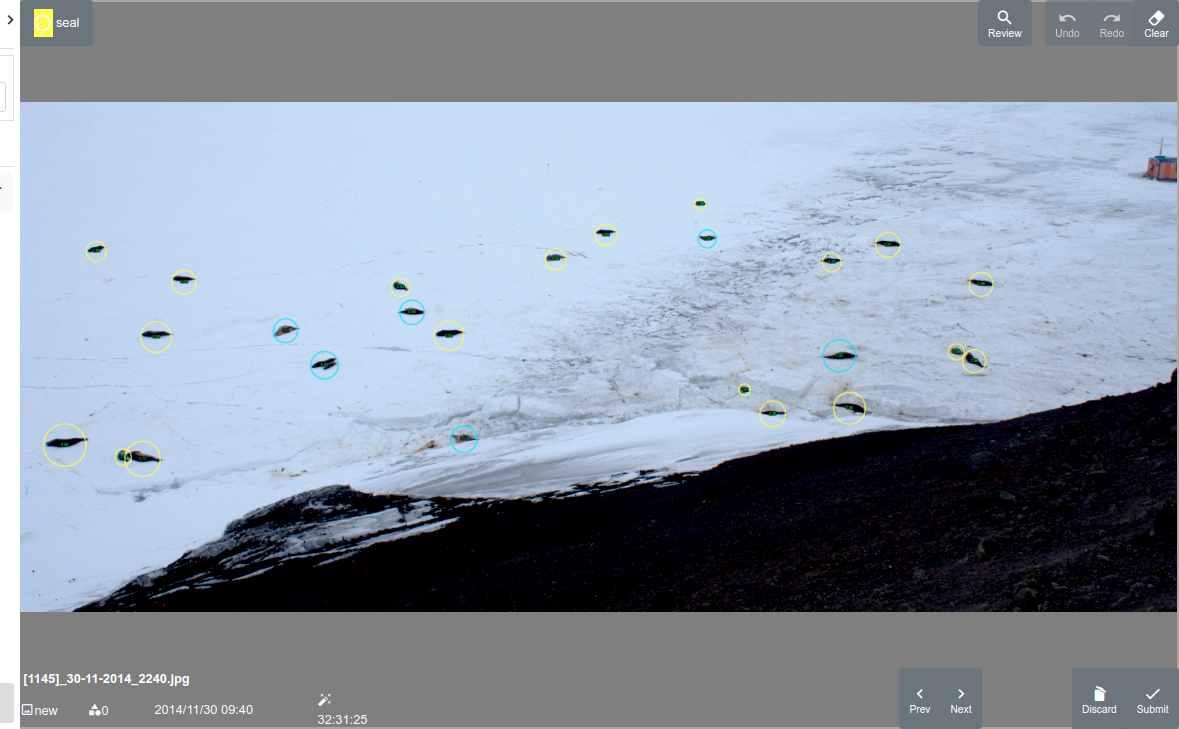
\includegraphics[width=0.475\linewidth]{figures/annotation/screenshots/seals_small.png}
  \caption{}
\end{subfigure}

\begin{subfigure}[t]{1.0\linewidth}
  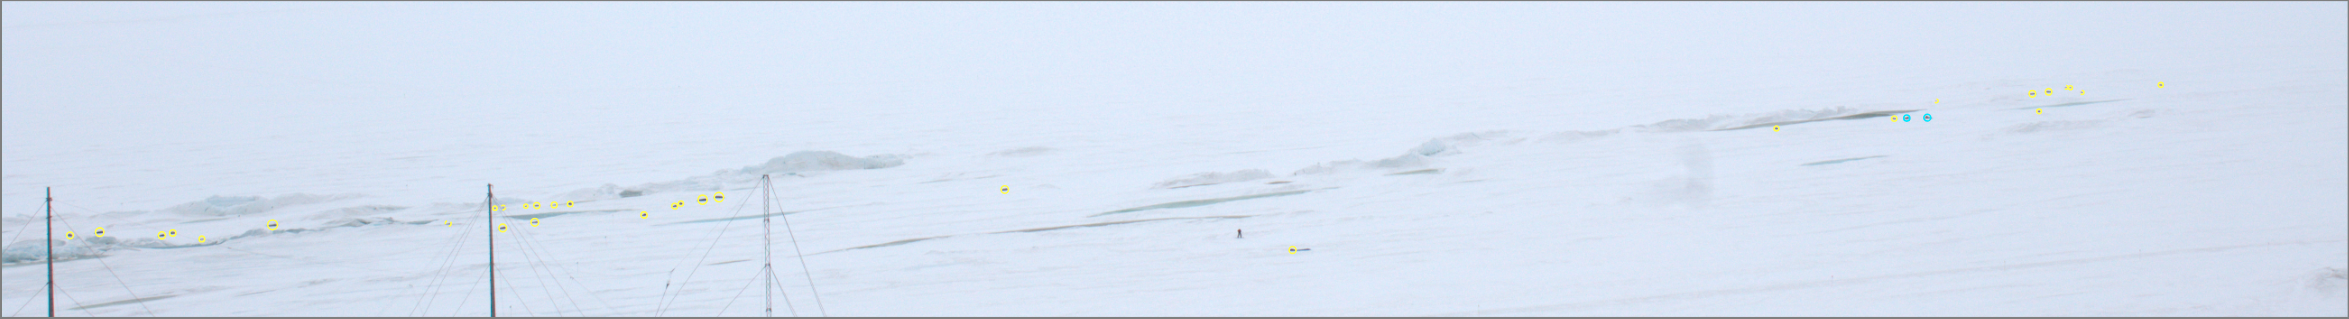
\includegraphics[width=1.0\linewidth]{figures/annotation/screenshots/cam_c.png}
\end{subfigure}

\begin{subfigure}[t]{1.0\linewidth}
  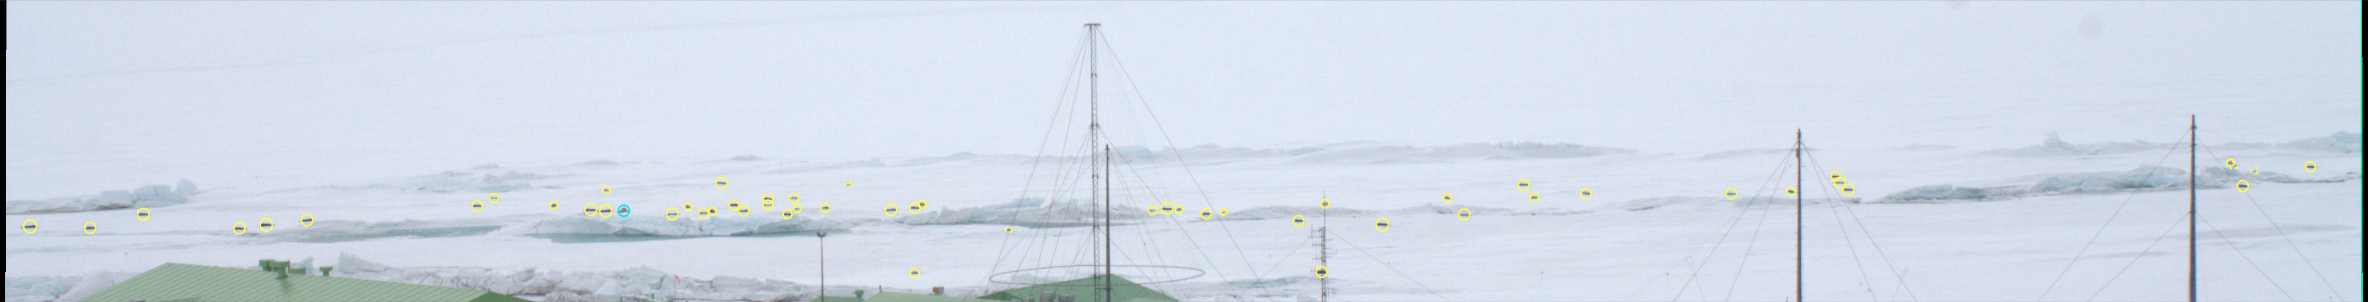
\includegraphics[width=1.0\linewidth]{figures/annotation/screenshots/cam_b.png}
  \caption{}
\end{subfigure}



\caption{ }
\label {fig:weddell_images}
\end{figure*}



\section{Discussion}


\subsection{Number of instances}
\label{sec:instances_discussion}

The instance distribution in each image has clear implications for verification based image annotation. Verifying several instances at once can be more efficient than one at a time, but verifying too many instances concurrently increases cognitive load (the very problem human in the loop machine learning seeks to address). 

Despite the ability to zoom into a small part of an image, in order to submit an image the user must review the whole image or remember which parts have been checked. For this reason when images become excessively large they should be split into pieces which can be easily verified without too much use of navigation.

This can be similar to a user interface for navigating search results, showing several results at once is much faster for a user to peruse than showing them one by one. However, if too many results are shown on each page results become lost in the crowd. A pair of studies found users do not look at results beyond 30 per page \cite{PunchoojitLumpapun2017, Zhou2007}.

The dual threshold approach helped in this regard by highlighting areas of uncertainty. For some datasets \emph{aerial penguins} and \emph{apples1}, \emph{apples2} the number of instances made it hard to keep track of progress when verifying the whole image. Combined with uncertain instances which are difficult to see without zooming, checking to ensure all annotations are present becomes difficult.

The dataset \emph{scott base} also suffers a little from this problem. The images are much wider than they are long, making navigation somewhat tedious and verifying the whole image much harder by having to zoom right out to check the whole image.

In future some method of marking parts of image as checked may help here.


